\section{\scshape Introduction}\label{sec:introduction}

\subsection{Context}
\begin{frame}{Context}
	\begin{itemize}
		\item Assembly of complex objects by robots requires long programming periods
		\item Most industrial robots are programmed to perform a very specific task in a controlled environment
		\begin{figure}[!ht]
			\centering
			\begin{minipage}{.35\textwidth}
				\centering
				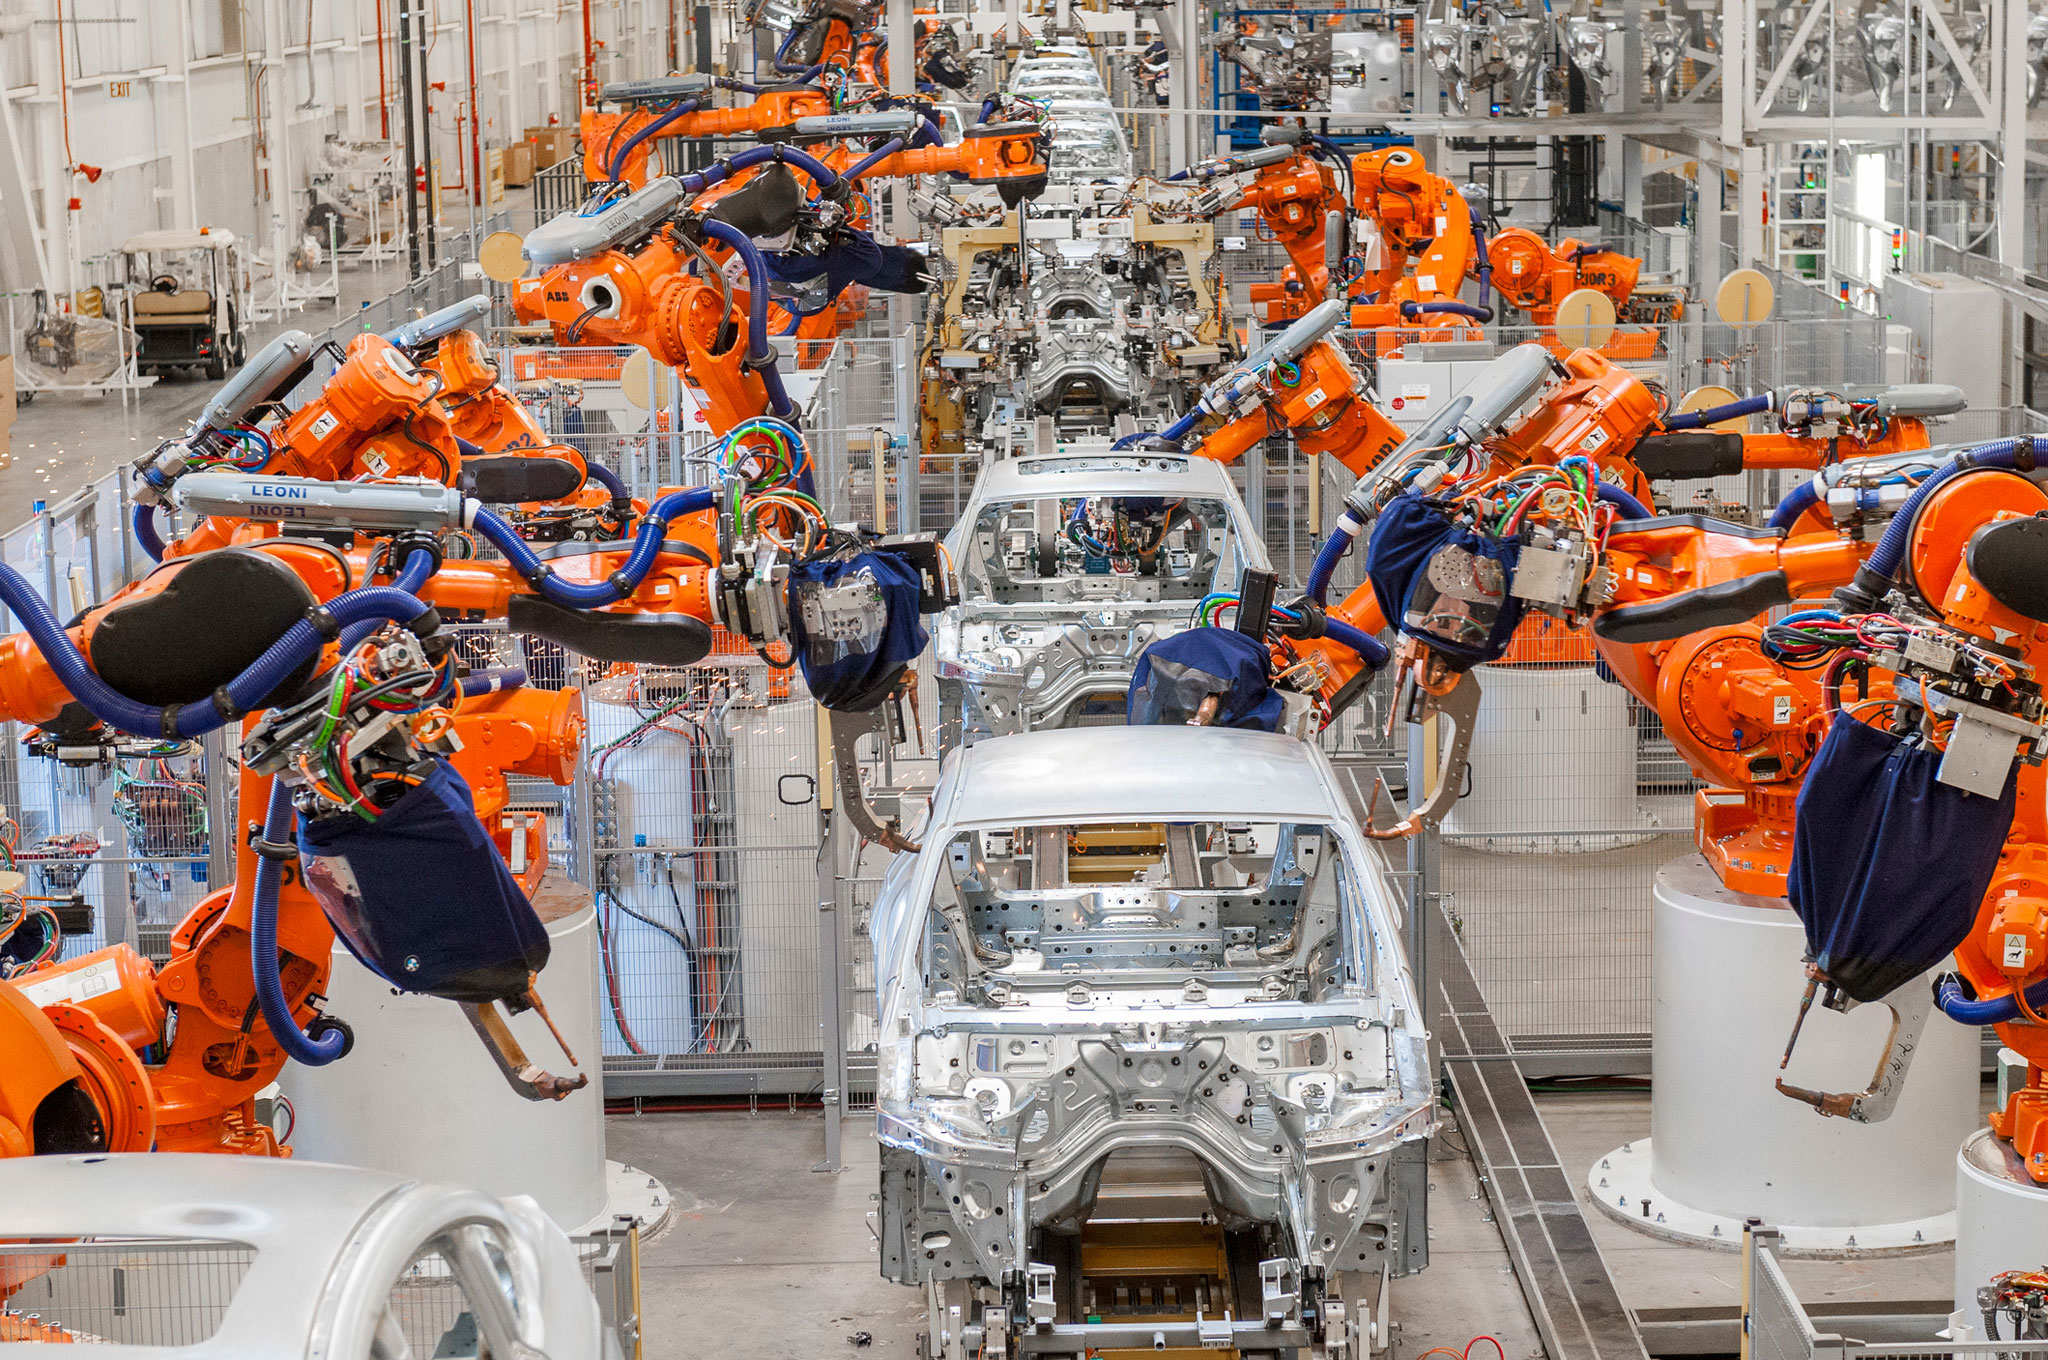
\includegraphics[height=.3\textheight]{bmw-spartanburg-robotic-welding-line}
				\caption{Car assembly line}
			\end{minipage}%
			\begin{minipage}{0.60\textwidth}
				\centering
				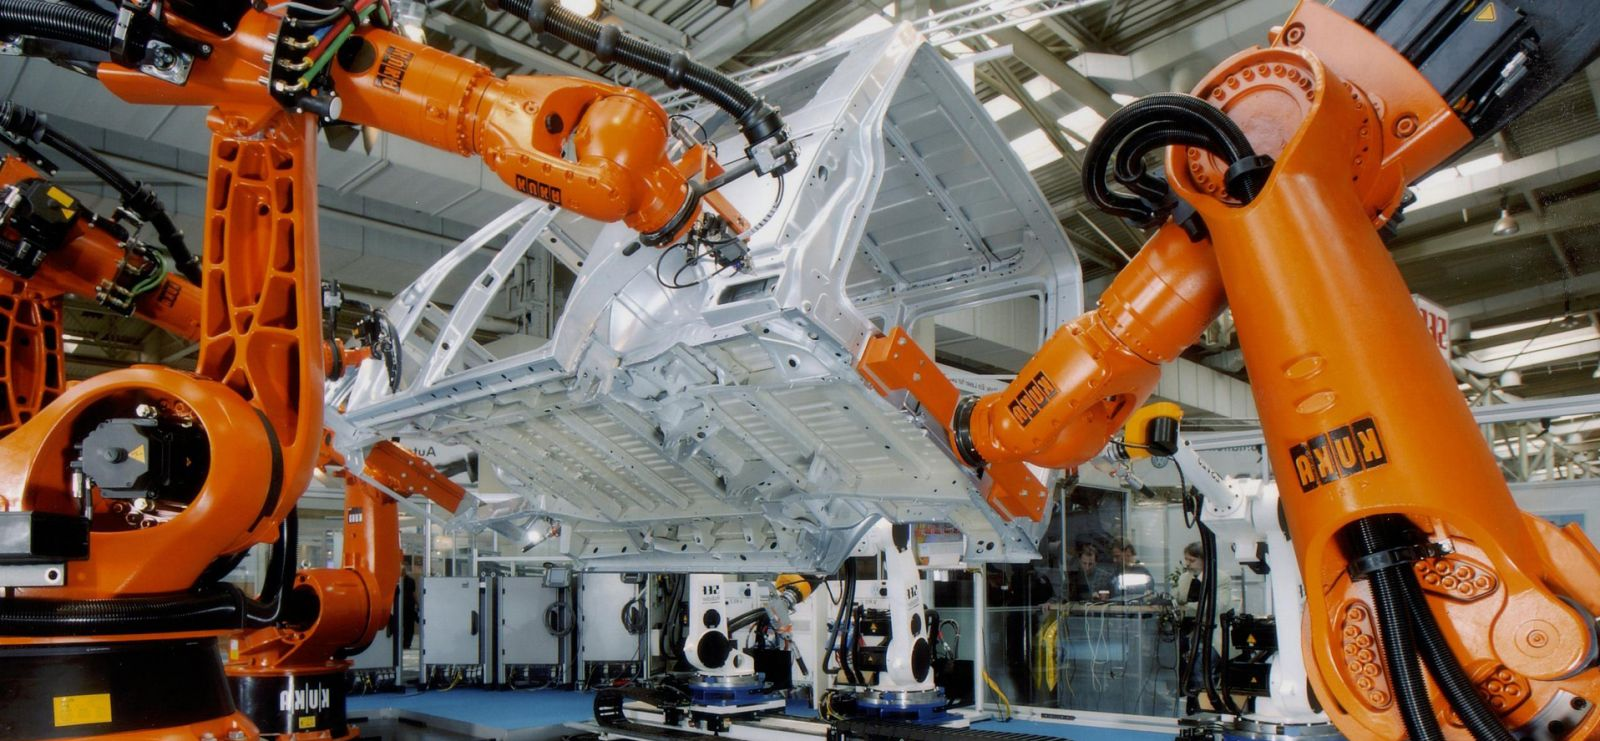
\includegraphics[height=.3\textheight]{kuka-heavy-assembly}
				\caption{Robots holding car}
			\end{minipage}
		\end{figure}
	\end{itemize}
\end{frame}


\subsection{Motivation}
\begin{frame}{Motivation}
	\begin{itemize}
		\item Teaching new assembly skills by demonstration can reduce the cost of re-purposing a robot for new tasks
		\item Cooperative assembly of complex objects can improve overall productivity
		\begin{itemize}
			\item Robot assembles components that it can quickly grasp and that need high assembly precision
			\item Human assembles the parts that the robot cannot grasp or the tasks that the robot takes more time than a human operator
		\end{itemize}
		\begin{figure}[!ht]
			\centering
			\begin{minipage}{.40\textwidth}
				\centering
				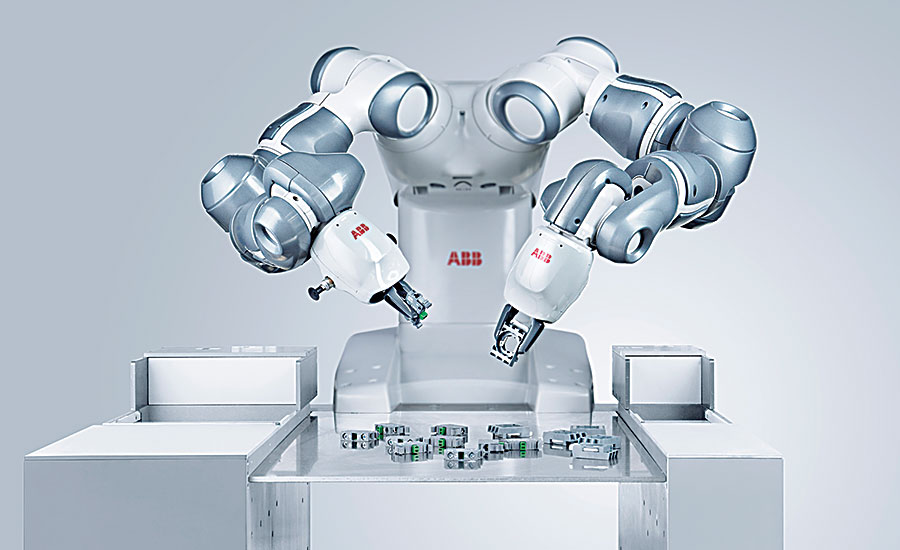
\includegraphics[height=.28\textheight]{yumi}
				\caption{ABB Yumi cooperative robot}
			\end{minipage}%
			\begin{minipage}{0.55\textwidth}
				\centering
				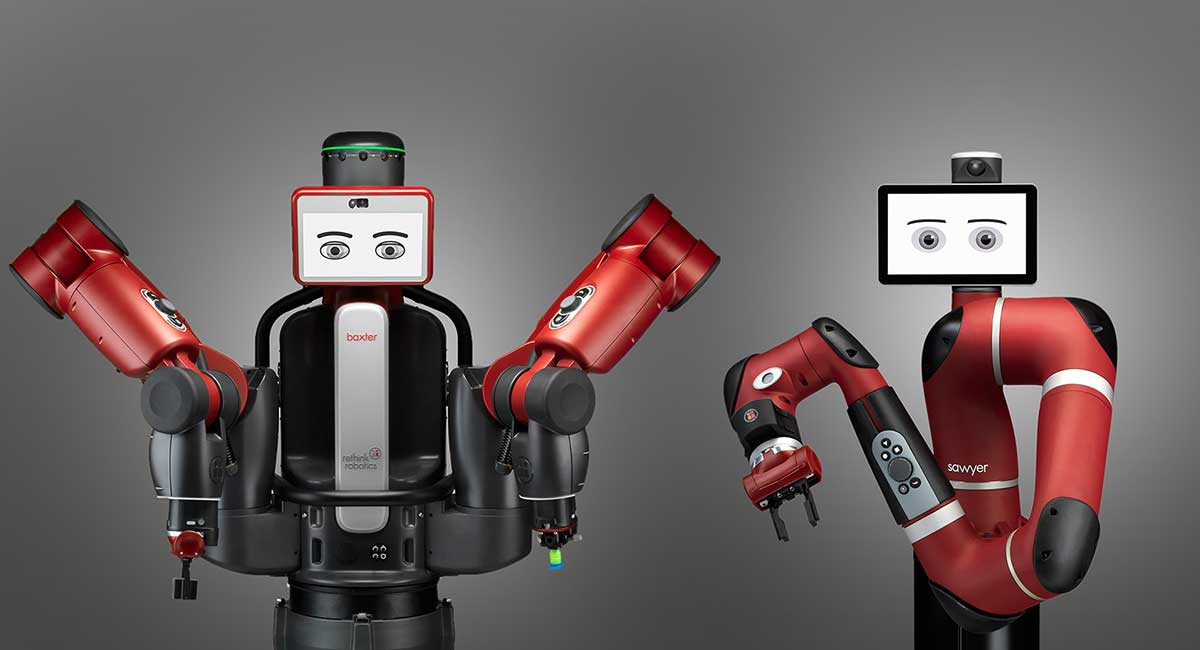
\includegraphics[height=.28\textheight]{rethink-robotics-baxter-sawyer}
				\caption{Rethink Robotics cooperative robots}
			\end{minipage}
		\end{figure}
	\end{itemize}
\end{frame}


\subsection{Research areas}
\begin{frame}{Research areas}
	\begin{itemize}
		\item Machine Learning
		\begin{itemize}
			\item Learning new semantic assembly skills by demonstration
		\end{itemize}
		\item Computer Vision, 3D perception and Human Machine Interface
		\begin{itemize}
			\item Recognition and tracking of assembly objects
			\item Detection of operator movements for semantic assembly analysis and user interface
			\item Human-robot cooperation
		\end{itemize}
		\item Augmented Reality
		\begin{itemize}
			\item Projection of information into the workspace to help the human operator
			\begin{itemize}
				\item Informing the operator which object it should pick and where it should assemble it
			\end{itemize}
		\end{itemize}
		\item Natural Language Processing
		\begin{itemize}
			\item Extraction of assembly information from instruction manuals
			\item Recognition of voice commands from the human operator
		\end{itemize}
	\end{itemize}
\end{frame}
